\documentclass[tikz,crop,border=10pt,multi]{standalone}
\usetikzlibrary{shapes.geometric}
\tikzset{my hexagon/.style={draw, minimum size=   4.000000 cm, regular polygon, regular polygon sides=6},}\begin{document}
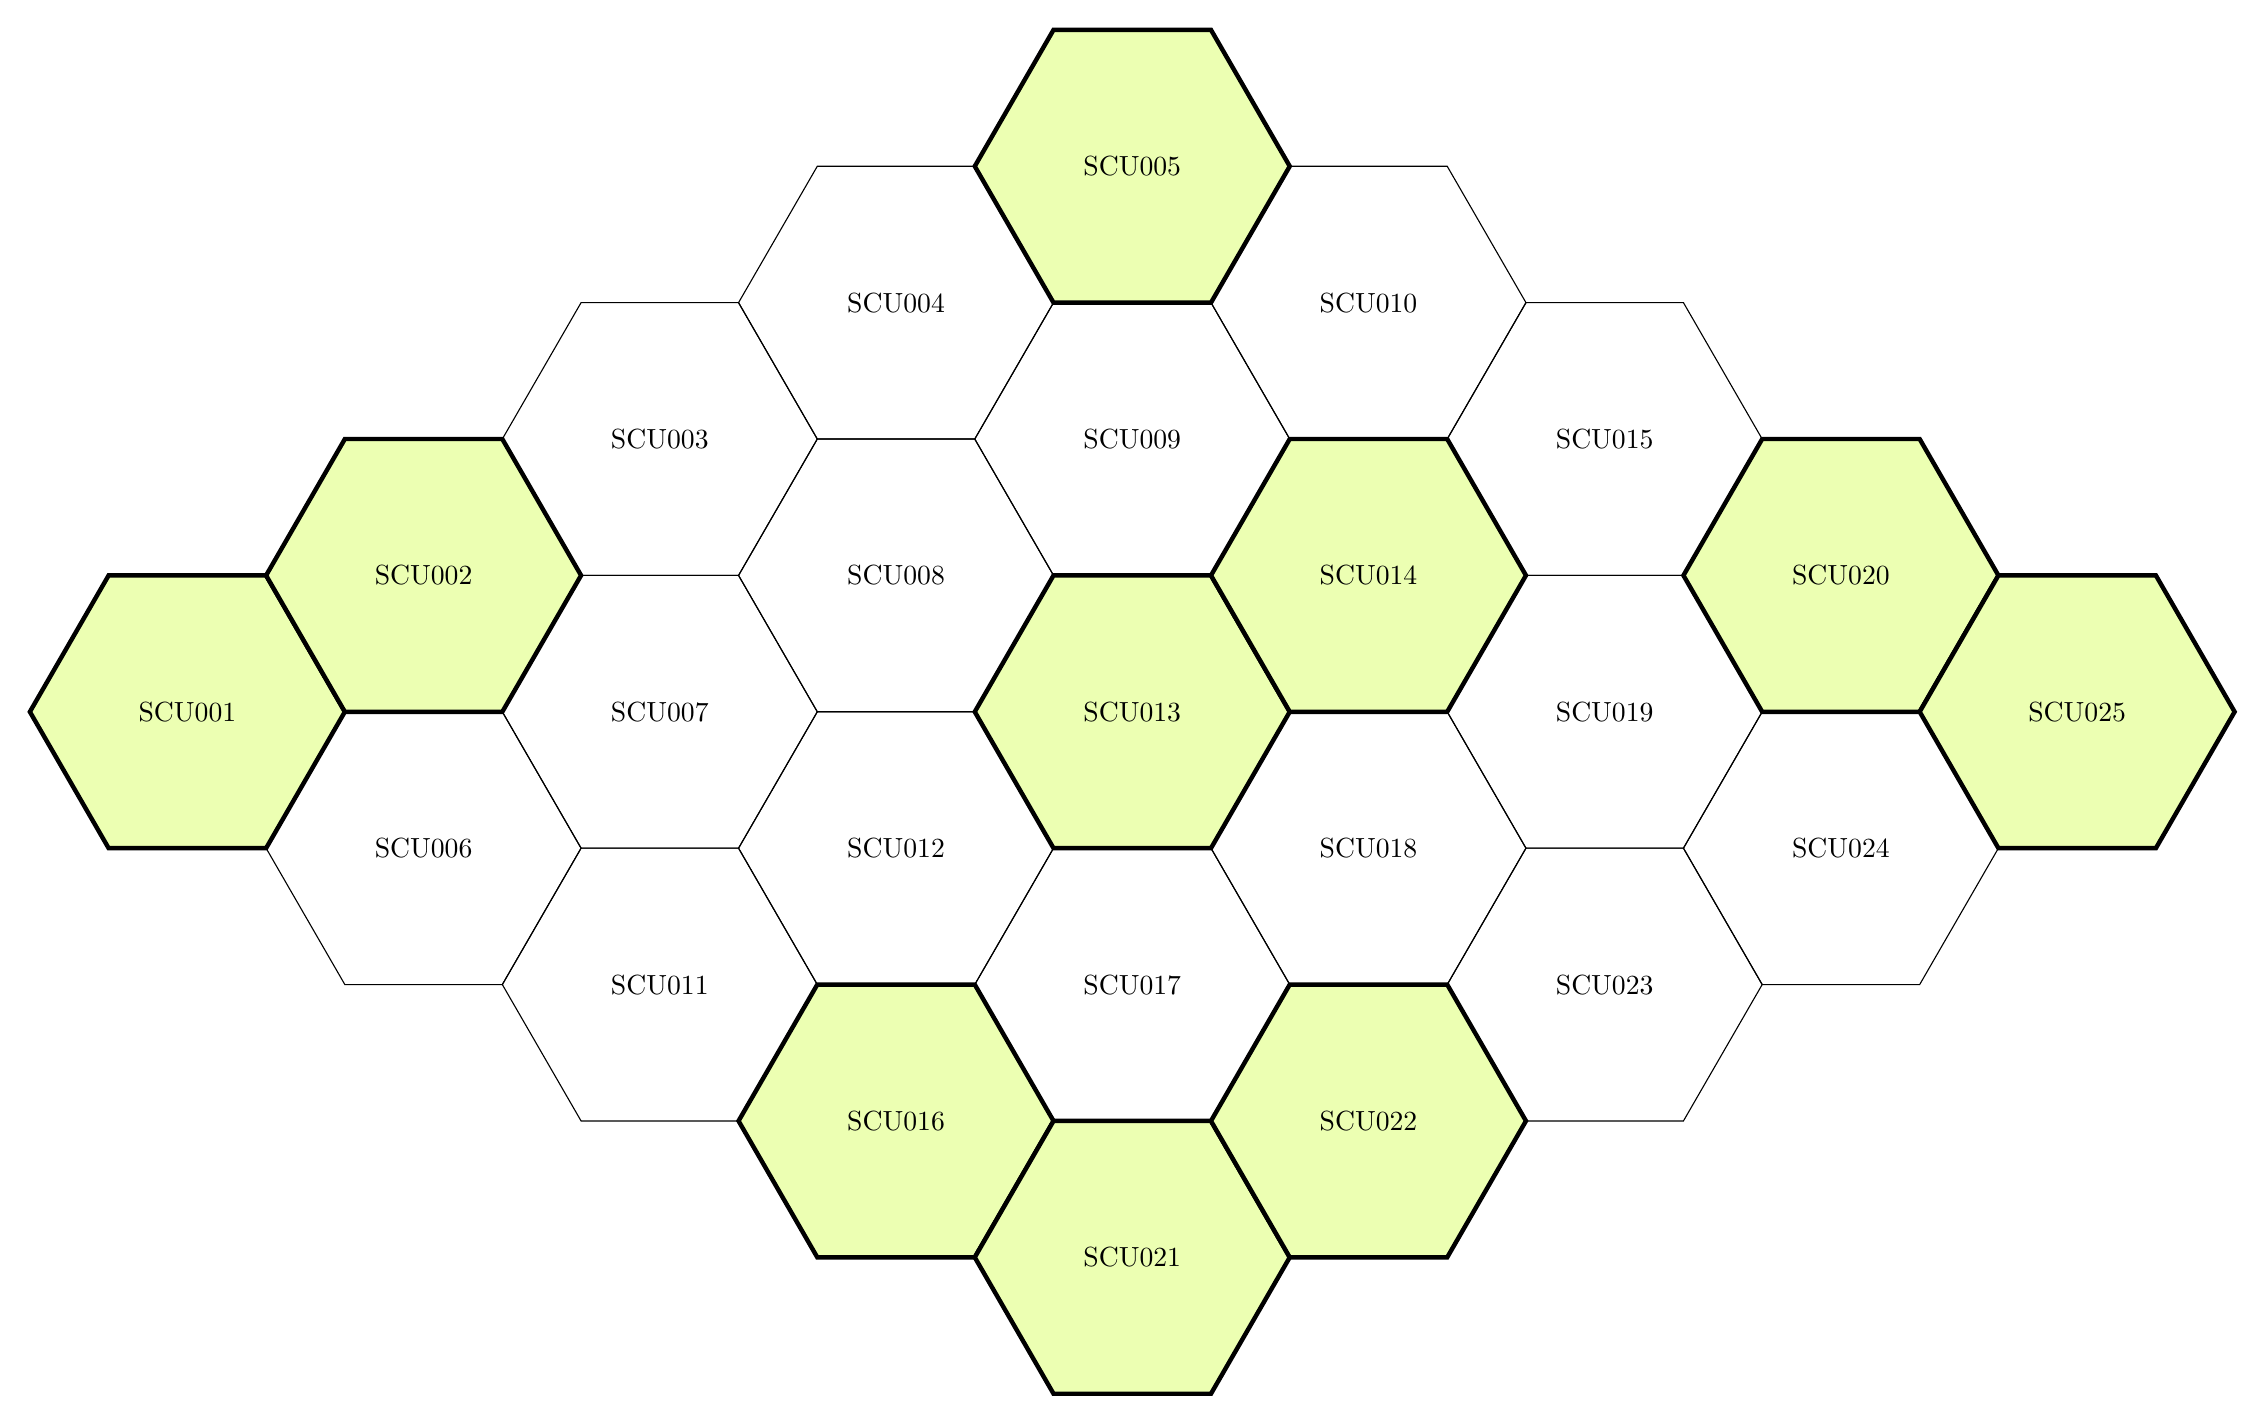
\begin{tikzpicture}
\node [my hexagon,ultra thick,fill = lime!30] at (  0.000000,  0.000000) {SCU001}; \\
\node [my hexagon,ultra thick,fill = lime!30] at (  3.000000,  1.732051) {SCU002}; \\
\node [my hexagon] at (  6.000000,  3.464102) {SCU003}; \\
\node [my hexagon] at (  9.000000,  5.196152) {SCU004}; \\
\node [my hexagon,ultra thick,fill = lime!30] at ( 12.000000,  6.928203) {SCU005}; \\
\node [my hexagon] at (  3.000000, -1.732051) {SCU006}; \\
\node [my hexagon] at (  6.000000,  0.000000) {SCU007}; \\
\node [my hexagon] at (  9.000000,  1.732051) {SCU008}; \\
\node [my hexagon] at ( 12.000000,  3.464102) {SCU009}; \\
\node [my hexagon] at ( 15.000000,  5.196152) {SCU010}; \\
\node [my hexagon] at (  6.000000, -3.464102) {SCU011}; \\
\node [my hexagon] at (  9.000000, -1.732051) {SCU012}; \\
\node [my hexagon,ultra thick,fill = lime!30] at ( 12.000000,  0.000000) {SCU013}; \\
\node [my hexagon,ultra thick,fill = lime!30] at ( 15.000000,  1.732051) {SCU014}; \\
\node [my hexagon] at ( 18.000000,  3.464102) {SCU015}; \\
\node [my hexagon,ultra thick,fill = lime!30] at (  9.000000, -5.196152) {SCU016}; \\
\node [my hexagon] at ( 12.000000, -3.464102) {SCU017}; \\
\node [my hexagon] at ( 15.000000, -1.732051) {SCU018}; \\
\node [my hexagon] at ( 18.000000,  0.000000) {SCU019}; \\
\node [my hexagon,ultra thick,fill = lime!30] at ( 21.000000,  1.732051) {SCU020}; \\
\node [my hexagon,ultra thick,fill = lime!30] at ( 12.000000, -6.928203) {SCU021}; \\
\node [my hexagon,ultra thick,fill = lime!30] at ( 15.000000, -5.196152) {SCU022}; \\
\node [my hexagon] at ( 18.000000, -3.464102) {SCU023}; \\
\node [my hexagon] at ( 21.000000, -1.732051) {SCU024}; \\
\node [my hexagon,ultra thick,fill = lime!30] at ( 24.000000,  0.000000) {SCU025}; \\
\end{tikzpicture}
\end{document}
